\chapter{Results}
This chapter shows the results and discussion for the following experiments.
% Reconstruction quality is mean of PSNR of images inside and outside of
% the training sets.
\begin{enumerate}
 \item Convergence of reconstruction quality for different dictionary sizes.
 \item Comparison of reconstruction quality of dictionaries
in single and in cluster runs. 
 \item Comparison of compression quality between learned dictionaries, JPEG and
JPEG2000  on natural images and sketches.
 \item Observations of structures of dictionary atoms from different
groups of images and block sizes.
\end{enumerate}


\newpage

\section{Training parameters}

Convergence of quality of different number of learning coefficients.
With high number of learning coefficents convergence is reached faster than
with a low number of coefficents but for large dicts fewer coefficents lead to
better reconstruction quality with larger training sets.


Convergence of quality of different block sizes.
But large blocks 


Quality
With single images learning, initialization with elements from training sets
improbes quality. but with large training set random data is works fine.

\begin{figure}[h]
\centering
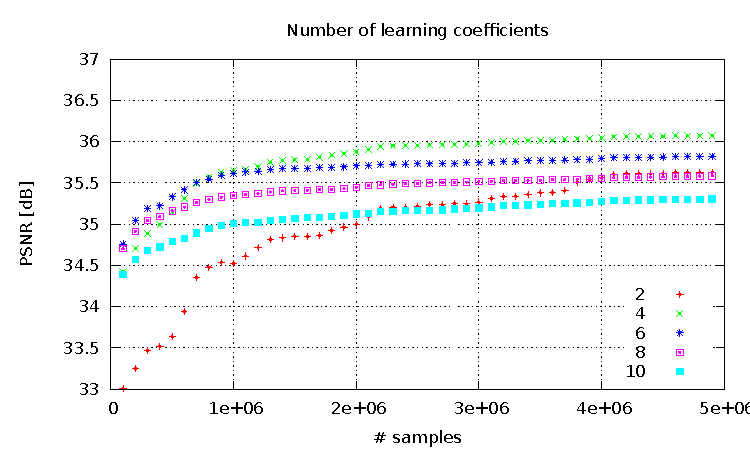
\includegraphics[width = 0.8\textwidth]{../tests/results/old/coeffsConverg.pdf}
\caption{reconstruction quality for different training coefficients (OMP)}
\label{fig:dict size}
\end{figure}

\begin{figure}[h]
\centering
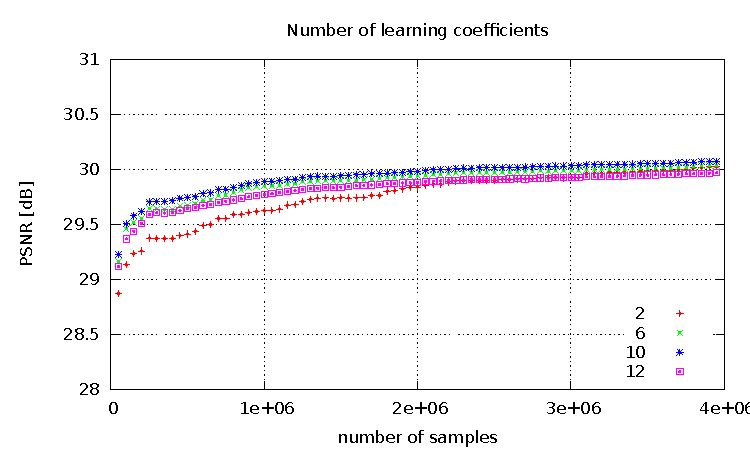
\includegraphics[width = 0.8\textwidth]{../tests/results/coeffsConverg.pdf}
\caption{reconstruction quality for different training coefficients (LARS)}
\label{fig:dict size}
\end{figure}

\begin{figure}[h]
\centering
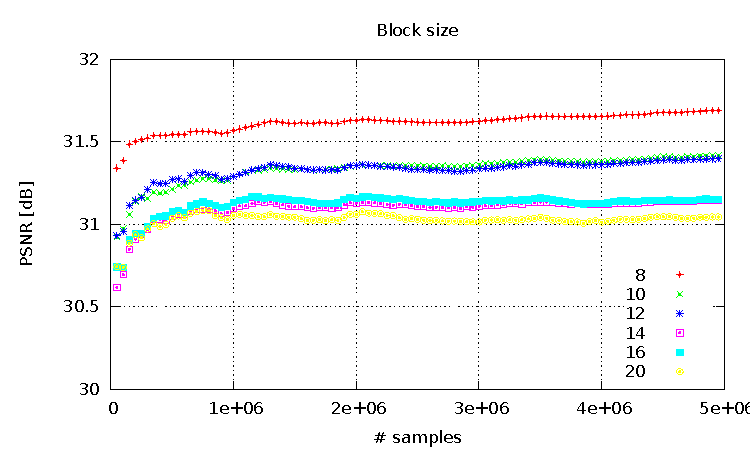
\includegraphics[width =
0.8\textwidth]{../tests/results/old/blockSizeConverg.pdf}
\caption{reconstruction quality for different block sizes}
\label{fig:dict size}
\end{figure}


\newpage
\section{Dictionary size}

\begin{figure}[h]
\centering
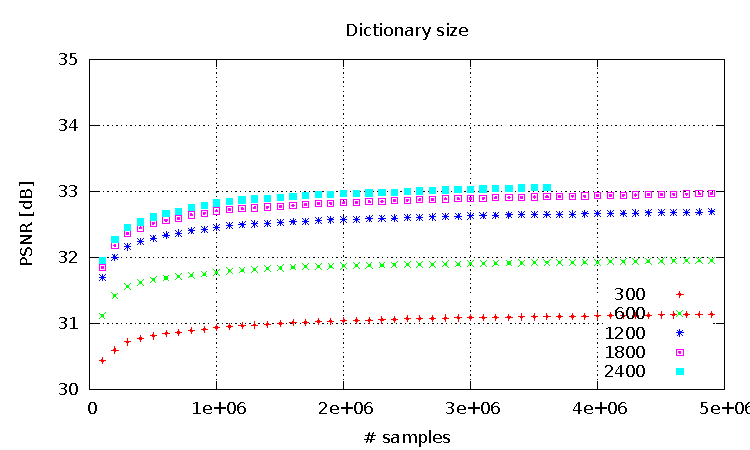
\includegraphics[width = 0.8\textwidth]{../tests/results/old/dictSizeOMP.pdf}
\caption{reconstruction quality for different dictionary sizes (OMP)}
\label{fig:dict size}
\end{figure}

\begin{figure}[h]
\centering
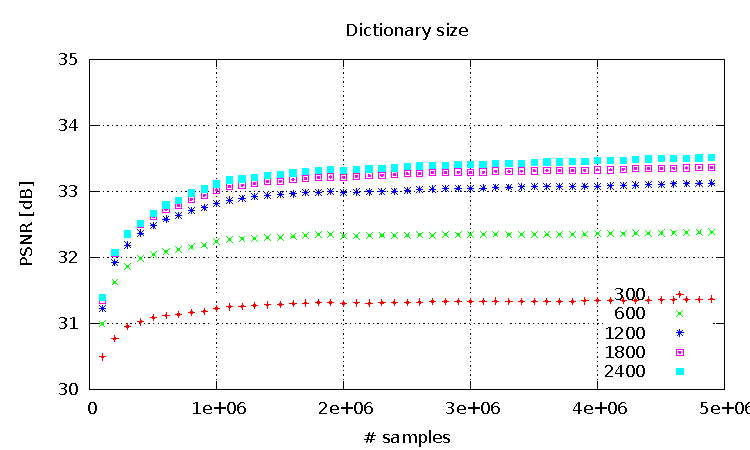
\includegraphics[width = 0.8\textwidth]{../tests/results/old/dictSizeLasso.pdf}
\caption{reconstruction quality for different dictionary sizes (Lasso)}
\label{fig:dict size}
\end{figure}


\newpage
\section{Compression}
Compression
For the short time available the results show promising results in visual
quality but still lack ...

Using LARS-Lasso for training generates a good dictionary for LARS and OMP. 
\Todo{ Training with OMP leads to a dictionary more with a lot of noise that
leads better coding results when using OMP.}


Difference in the selection strategy.
Very noisy vs. smooth. 
How this different selection strategies affect the learning step will be
presented in the next section.
\subsection{Natural images}

\begin{figure}[h]
\centering
\subfloat{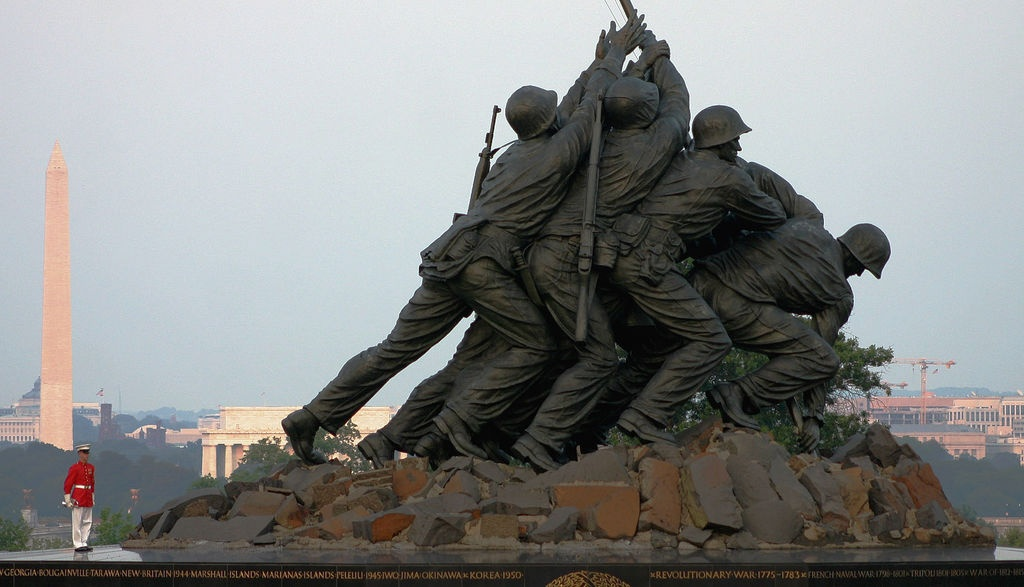
\includegraphics[width = 0.3\textwidth]{images/28979823.jpg}}
\hspace{5mm}
\subfloat{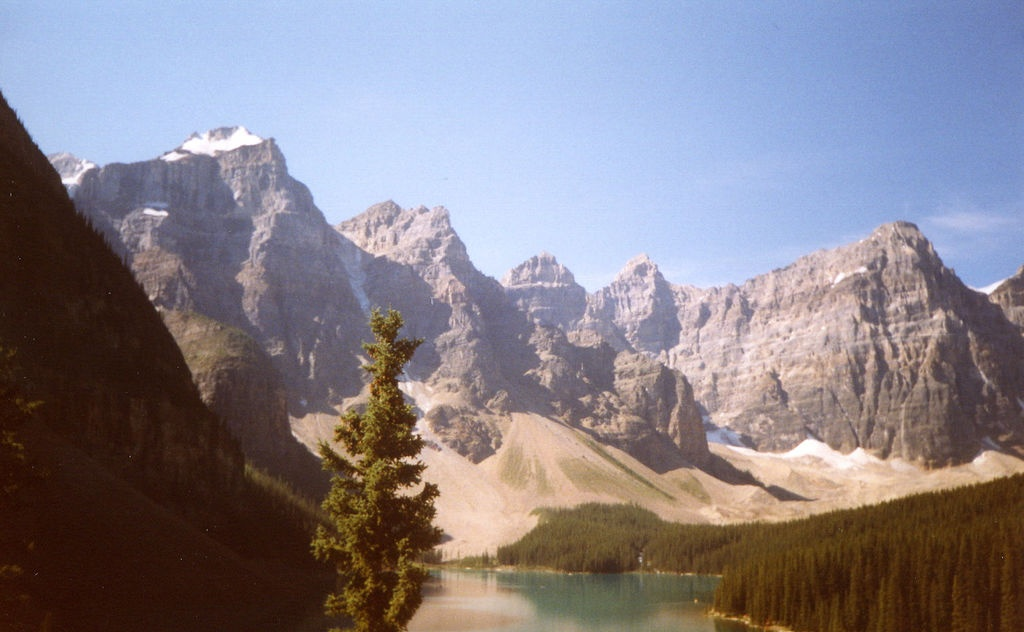
\includegraphics[width = 0.3\textwidth]{images/29018694.jpg}}
\hspace{5mm}
\subfloat{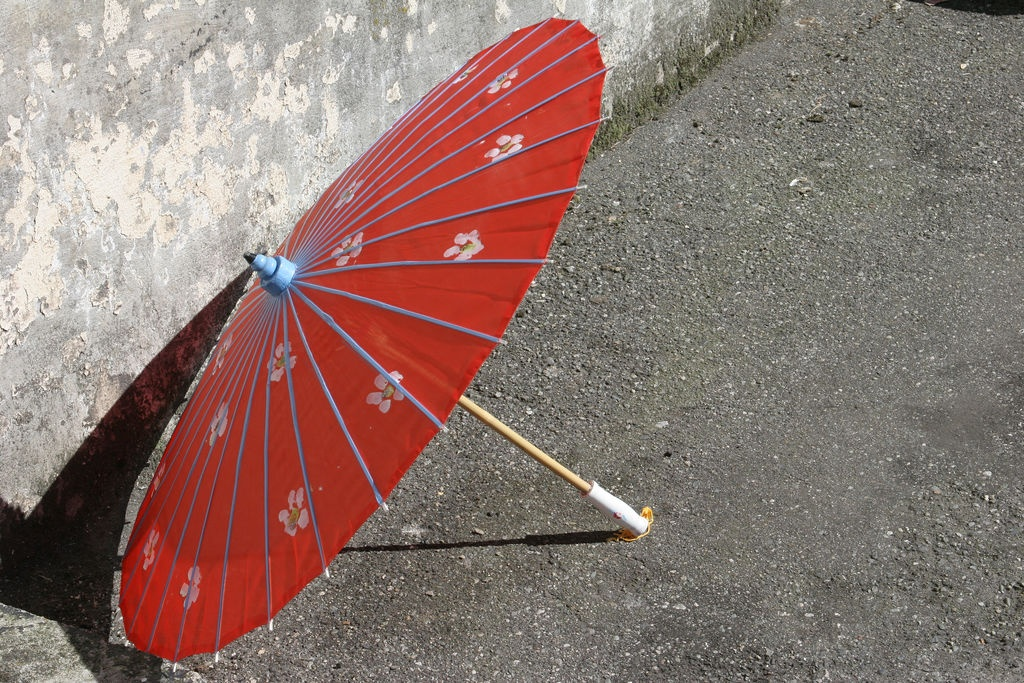
\includegraphics[width = 0.3\textwidth]{images/28874882.jpg}}
\hspace{5mm}
\subfloat{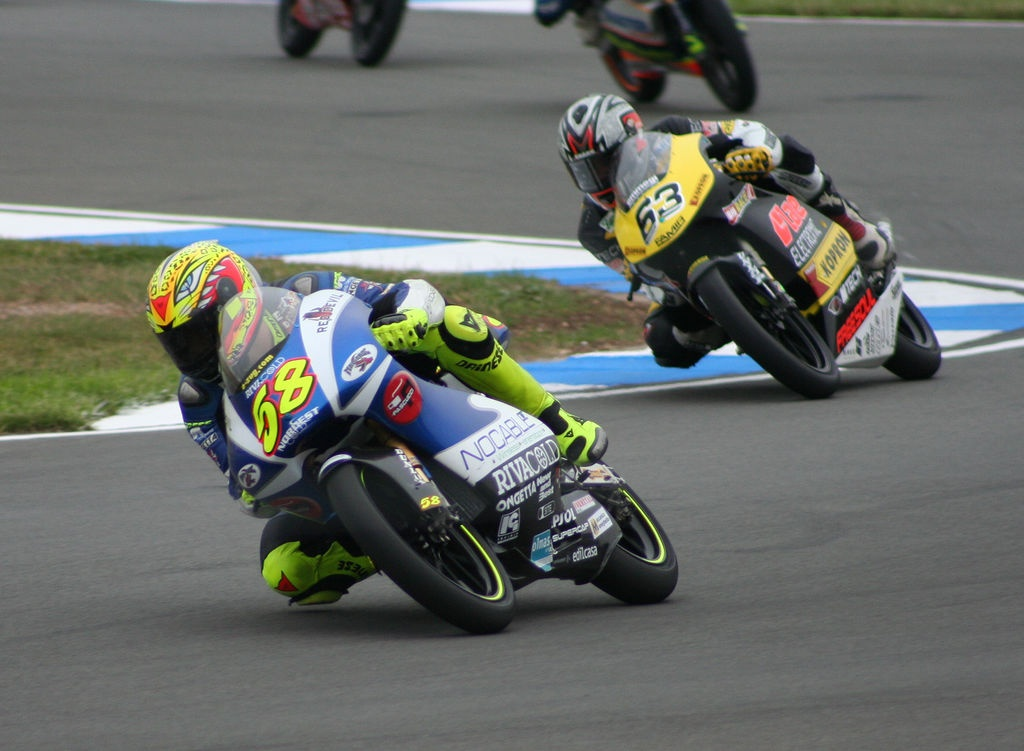
\includegraphics[width = 0.3\textwidth]{images/28803842.jpg}}
\hspace{5mm}
\subfloat{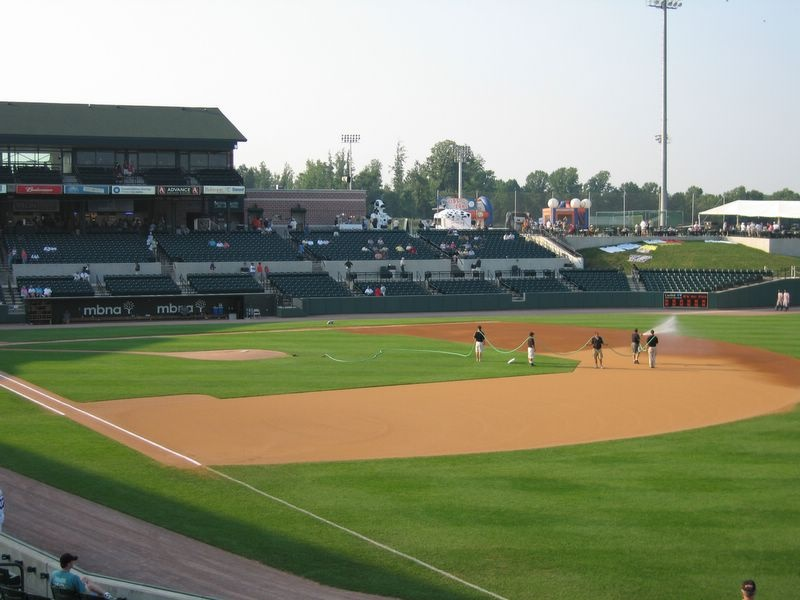
\includegraphics[width = 0.3\textwidth]{images/28894495.jpg}}
\hspace{5mm}
\subfloat{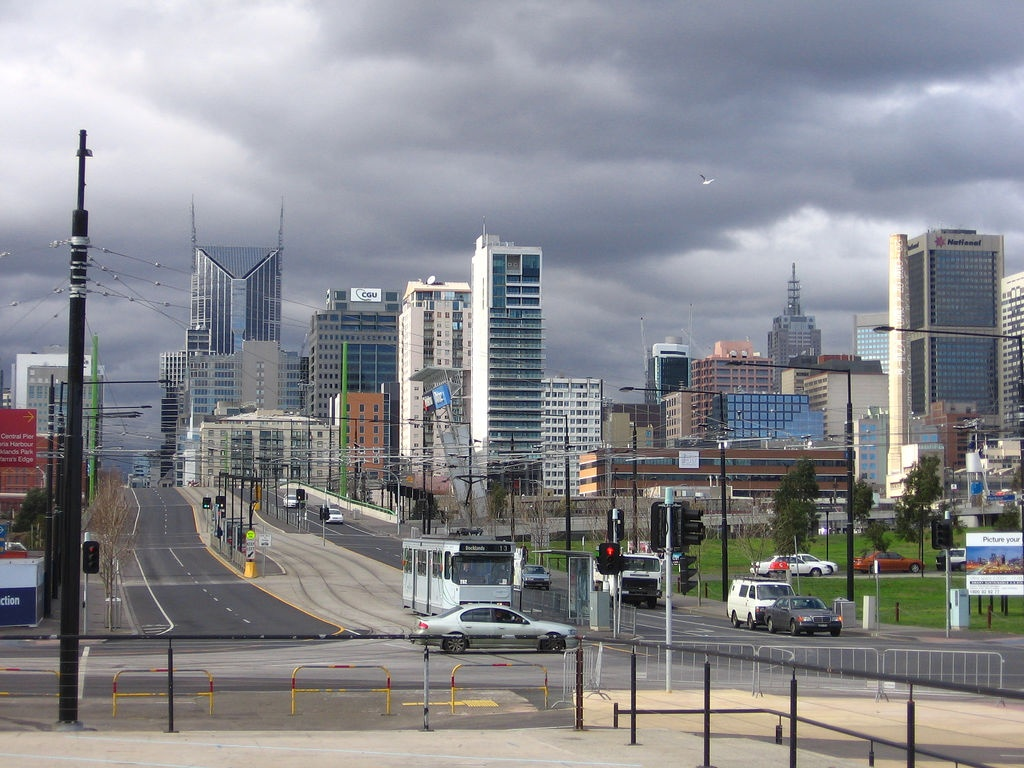
\includegraphics[width = 0.3\textwidth]{images/28952841.jpg}}
\caption{test images from training set}
\label{fig:database_images}
\end{figure}

\begin{table}[H]
%\caption{single vs. cluster}
\centering
\begin{tabular}{| l c | c | c | c|}
\hline\hline
Image & bpp & SPRS & JPEG & JPEG2000 \\
\hline
image 1 & 1.12 & 31.2205 & 32.3289 & 36.613 \\
image 2 & 1.01 & 34.7735 & 35.0671 & 40.3299 \\
image 3 & 1.8  & 29.0597 & 27.2556 & 31.7412 \\
image 4 & 0.74  & 35.9499 & 35.5104 & 39.4195 \\

\hline
\end{tabular}
\end{table}

\begin{figure}[H]
\centering
\subfloat[sprs ]{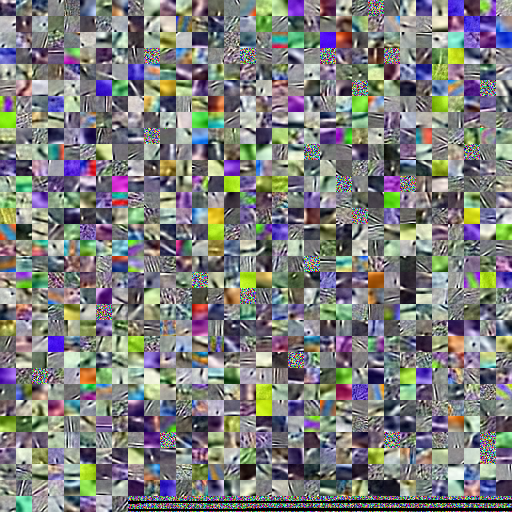
\includegraphics[width =
0.3\textwidth]{images/16_1000_1000_10_lasso.png}}
\hspace{5mm}
\subfloat[JPEG]{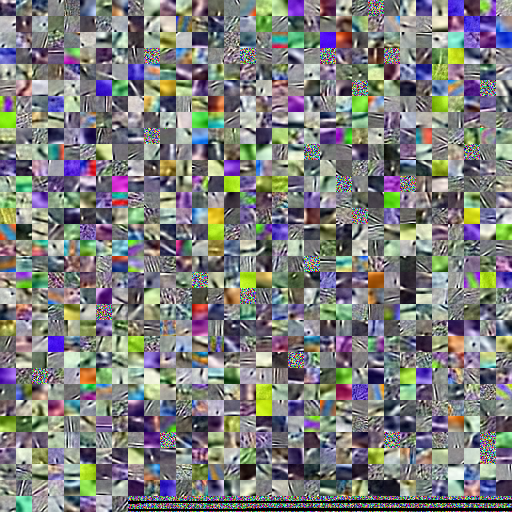
\includegraphics[width =
0.3\textwidth]{images/16_1000_1000_10_lasso.png}}
\hspace{5mm}
\subfloat[JPEG2000]{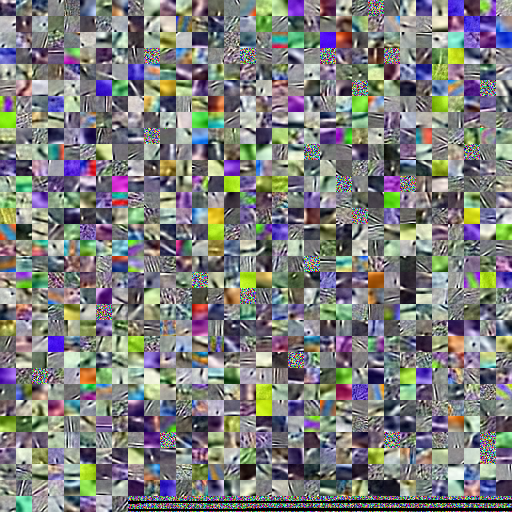
\includegraphics[width =
0.3\textwidth]{images/16_1000_1000_10_lasso.png}}
%\caption{}
%\label{fig:16_1000_lasso}
\end{figure}

\begin{figure}[H]
\centering
\subfloat[sprs]{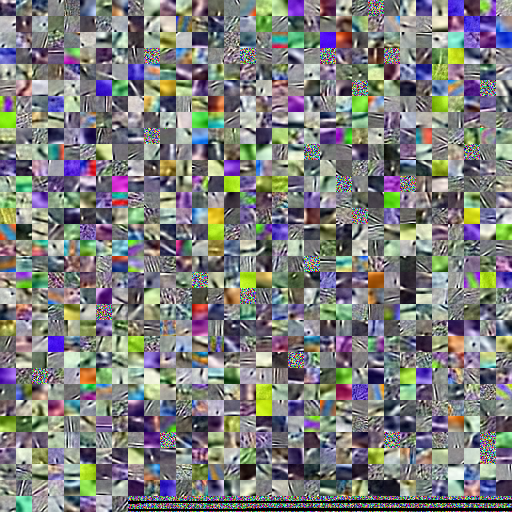
\includegraphics[width =
0.3\textwidth]{images/16_1000_1000_10_lasso.png}}
\hspace{5mm}
\subfloat[JPEG]{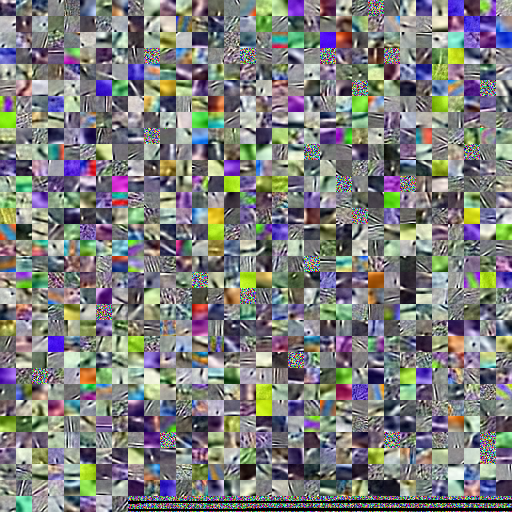
\includegraphics[width =
0.3\textwidth]{images/16_1000_1000_10_lasso.png}}
\hspace{5mm}
\subfloat[JPEG2000]{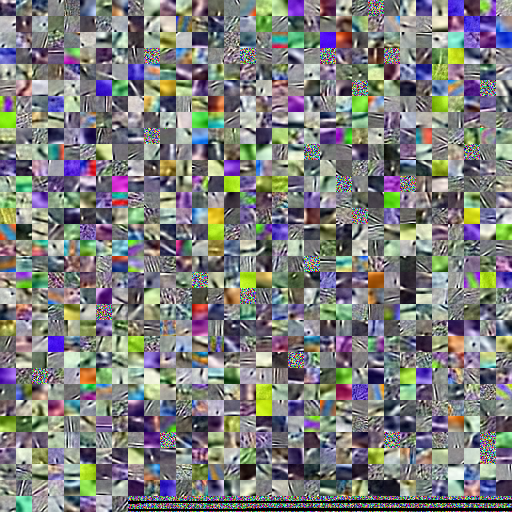
\includegraphics[width =
0.3\textwidth]{images/16_1000_1000_10_lasso.png}}
%\caption{}
%\label{fig:16_1000_lasso}
\end{figure}



\newpage
\subsection{Sketches}

\begin{figure}[h]
\centering
\setcounter{subfigure}{0}
\subfloat[]{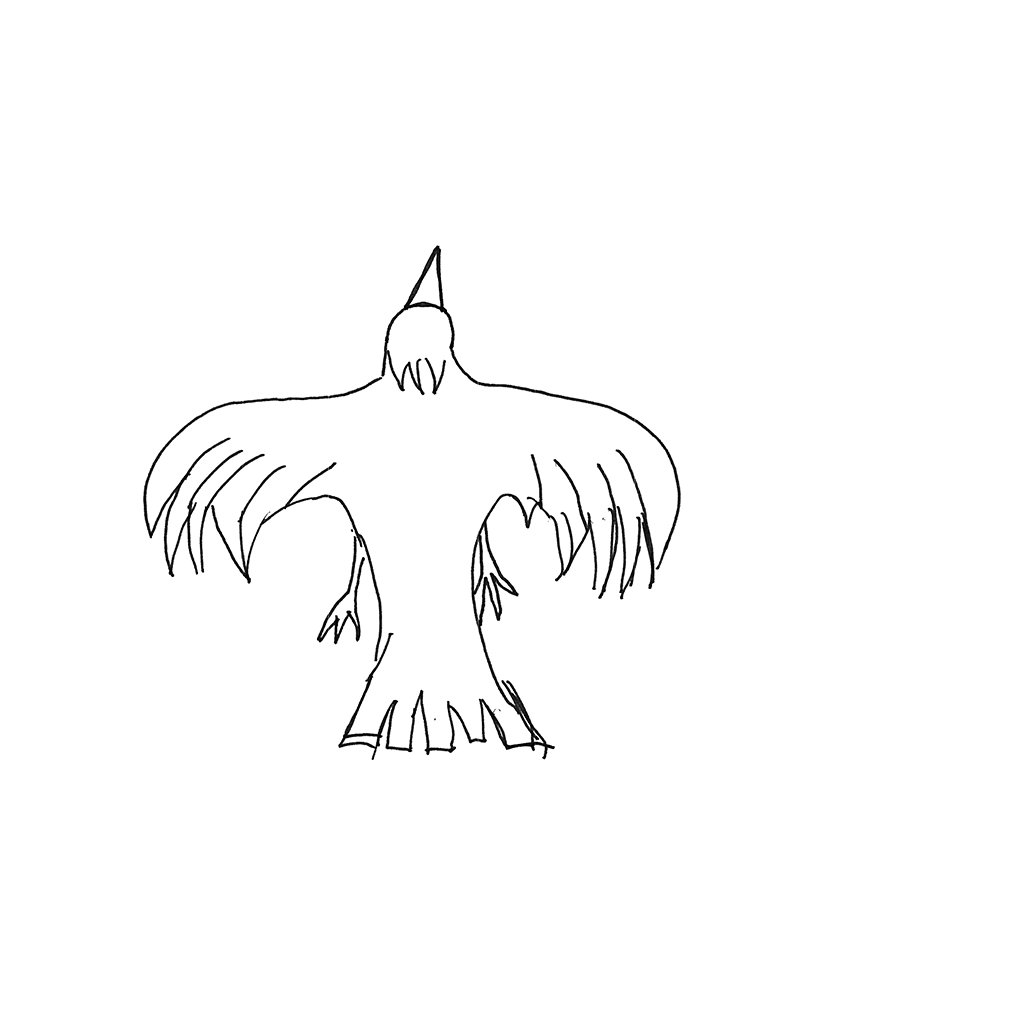
\includegraphics[width =
0.3\textwidth]{images/sketch1.jpg}}
\hspace{5mm}
\subfloat[]{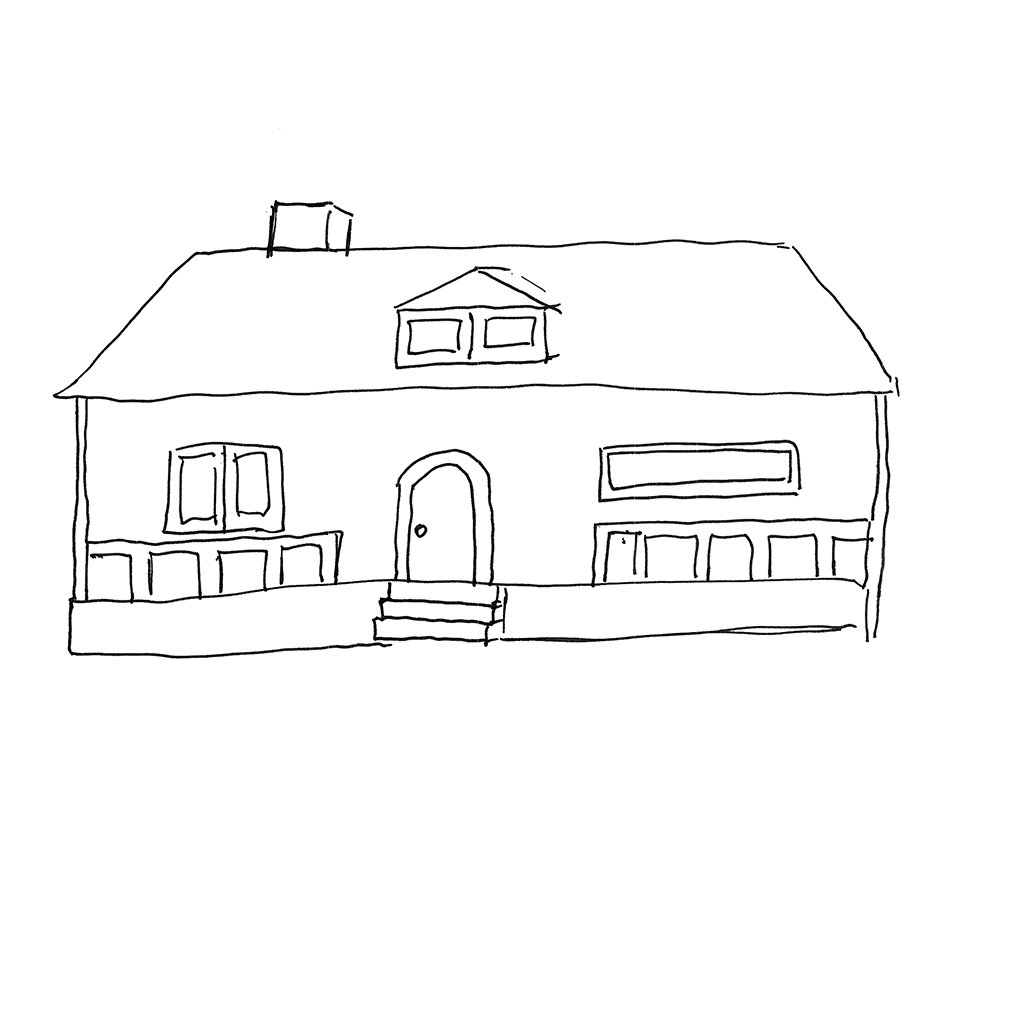
\includegraphics[width = 0.3\textwidth]{images/sketch2.jpg}}
\hspace{5mm}
\subfloat[]{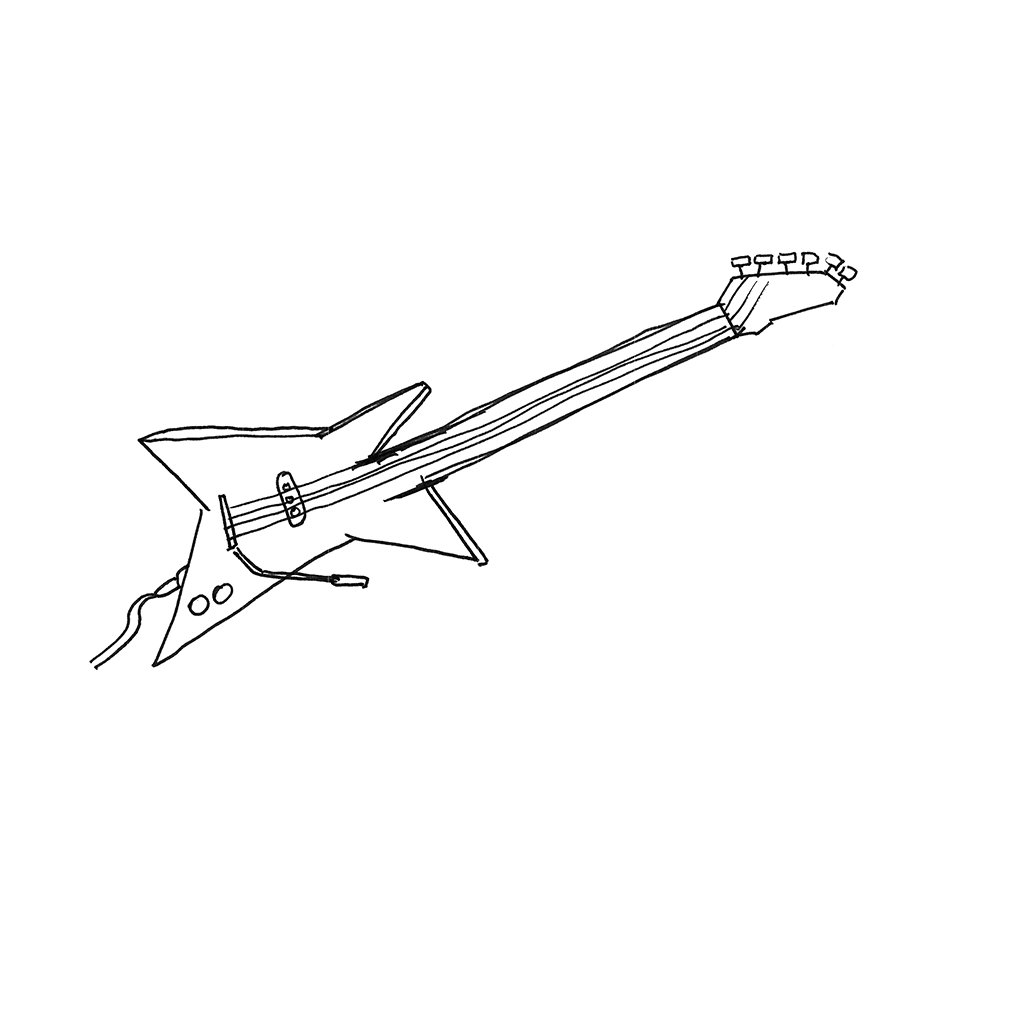
\includegraphics[width = 0.3\textwidth]{images/sketch3.jpg}}
\hspace{5mm}
\caption{sketches}
\label{fig:sketches}
\end{figure}


\begin{table}[H]
%\caption{single vs. cluster}
\centering
\begin{tabular}{| c c | c | c | c|}
\hline\hline
Image & bpp & SPRS & JPEG & JPEG2000 \\
\hline
a & 0.084 & 33.9594 & 28.9578 & 38.3258  \\
b & 0.13 & 32.9 & 34.5546 &  40.0159 \\
c & 0.08 & 32.5131 & 28.6558 & 36.3093  \\
\hline
\end{tabular}
\end{table}

\begin{figure}[H]
\centering
\subfloat[sprs]{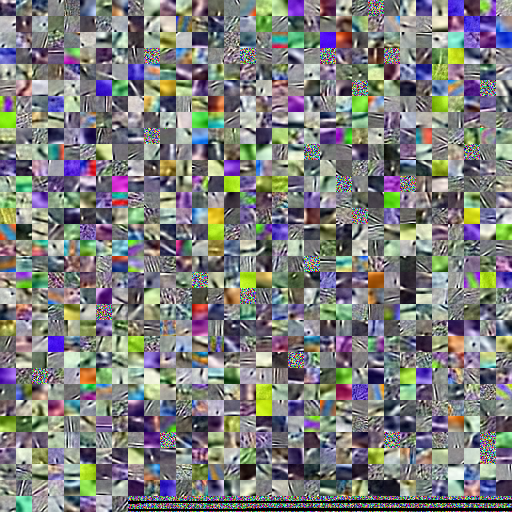
\includegraphics[width =
0.3\textwidth]{images/16_1000_1000_10_lasso.png}}
\hspace{5mm}
\subfloat[JPEG]{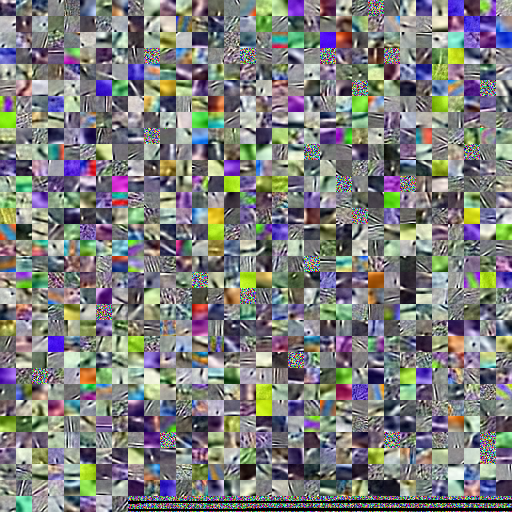
\includegraphics[width =
0.3\textwidth]{images/16_1000_1000_10_lasso.png}}
\hspace{5mm}
\subfloat[JPEG2000]{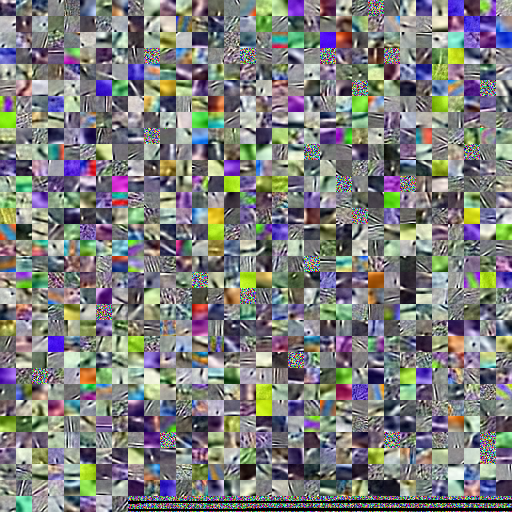
\includegraphics[width =
0.3\textwidth]{images/16_1000_1000_10_lasso.png}}
%\caption{}
%\label{fig:16_1000_lasso}
\end{figure}

\begin{figure}[H]
\centering
\subfloat[sprs]{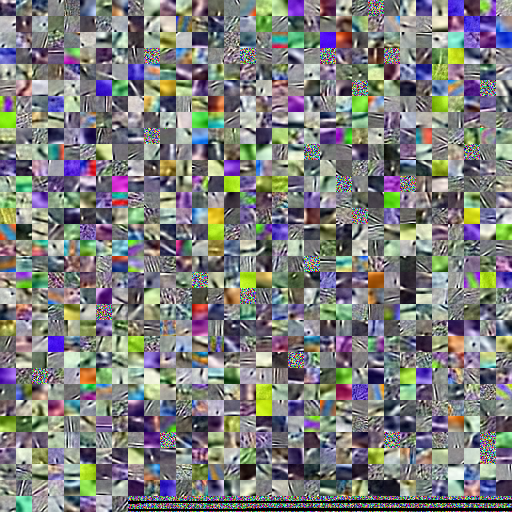
\includegraphics[width =
0.3\textwidth]{images/16_1000_1000_10_lasso.png}}
\hspace{5mm}
\subfloat[JPEG]{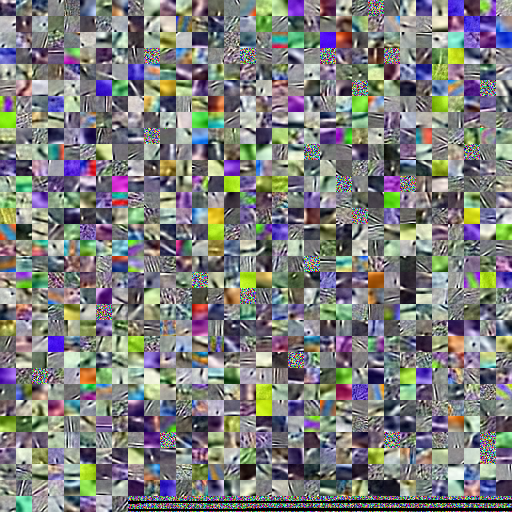
\includegraphics[width =
0.3\textwidth]{images/16_1000_1000_10_lasso.png}}
\hspace{5mm}
\subfloat[JPEG2000]{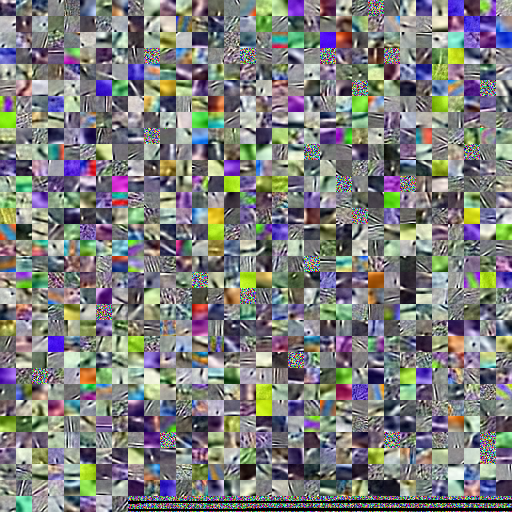
\includegraphics[width =
0.3\textwidth]{images/16_1000_1000_10_lasso.png}}
%\caption{}
%\label{fig:16_1000_lasso}
\end{figure}



\newpage
\section{Dictionary elements}
Appearance 
Learn basis similar to DCT and wavelets/bandelets(time and freq locality) with
increasing block size. Use to verify if it is a jpeg image?
Similar to natural images.
compression dicts
Dictionaries to universal ... improved results to DCT .. but varying with field
of application. possible no universal solution but a good way for better
understanding of the key elements
  four major types of elements
  gradient, checkerboard (low color more b/w), spot, edge
Better understanding the selection strategies of the algorithm and their
meaning for perceptional image quality. And evolution of the structure of
learned dictionaries. 

\begin{figure}[H]
\centering
\subfloat{
\includegraphics[width = 0.3\textwidth]{images/gradient.png}}
\hspace{5mm}
\subfloat{
\includegraphics[width = 0.3\textwidth]{images/checkerboard.png}}
\hspace{5mm}
\subfloat{
\includegraphics[width = 0.3\textwidth]{images/spot.png}}
\hspace{5mm}
\subfloat{
\includegraphics[width = 0.3\textwidth]{images/edges.png}}
\hspace{5mm}
\subfloat{
\includegraphics[width = 0.3\textwidth]{images/wavelet.png}}
\caption{image from database}
\label{fig:USC-SIPI}
\end{figure}





